\documentclass[11pt]{article}
% PACKAGES
%  various packages that you may wish to activate for usage 
\usepackage{graphicx}
\usepackage{tabls}
\usepackage{afterpage}
\usepackage{amsmath}
\usepackage{amsfonts}
\usepackage{amssymb}
\usepackage{amstext}
\usepackage{amsbsy}
\usepackage{epsfig}
%\usepackage{cites}
\usepackage{epsf}
\usepackage{float} %utiliser H pour forcer � mettre l'image o� on ve

\usepackage{array}
{\usepackage{color}}
\usepackage[section]{placeins} % force � mettre l'image o� on veut
\usepackage{lscape} %utilisation du mode paysage
\usepackage{xspace}

%\usepackage[pdftex,bookmarks=true]{hyperref}
%\usepackage{hyperref}
\usepackage{url}
\usepackage{verbatim}
%\usepackage[all]{hypcap}

\usepackage[labelsep=quad]{caption} % needed by the breakalgo environment

\usepackage{ifthen}
\usepackage{subfig}

\usepackage{algorithmic}
\usepackage{algorithm}
\usepackage{listings}
\usepackage[noprefix]{nomencl}  % for nomenclature
%\usepackage[intoc]{nomencl}  % for nomenclature

%\usepackage{notebook2e, latexsym}
%
% de dk:
%
%%\usepackage[dvips]{epsfig}
%%\usepackage[dvips]{graphicx}
%%\usepackage{comment}
%%\usepackage{floatfig}
%%\usepackage{lscape}
%%\usepackage{landscape}
%%\usepackage{graphics}
%%\usepackage{hhline}[]
%%\usepackage{latexsym}
%%\usepackage{tabularx}[]
%%\usepackage{layout}
%
% de btp:
%
%%\usepackage{fancyheadings}
%%\usepackage{minitoc}
\usepackage{rotating}
%% \usepackage{rotate}
%%\usepackage{subfigure}
%%\usepackage{mathaccent}
%%\usepackage{isolatin1}
%
%%\usepackage{xspace}
%%\usepackage{longtable}
%%\usepackage{caption2}
%%\usepackage{ifthen}
%
\usepackage{graphics}
\usepackage{graphicx}
\usepackage{color}
%-----------------------------------------------------------
% NEW  DEFINITIONS
%
%=================================================================================================
% new commands
% +++++++++++++++++++++++++++++++++++++++++++++++++++++++++++++++++++++++++++++++++++++++++++++++++
\newcommand{\nc}{\newcommand}
%
% Ways of grouping things
%
\newcommand{\bracket}[1]{\left[ #1 \right]}
\newcommand{\bracet}[1]{\left\{ #1 \right\}}
\newcommand{\fn}[1]{\left( #1 \right)}
\newcommand{\ave}[1]{\left\langle #1 \right\rangle}
%
% Derivative forms
% 
\newcommand{\dx}[1]{\,d#1}
\newcommand{\dxdy}[2]{\frac{\partial #1}{\partial #2}}
\newcommand{\dxdt}[1]{\frac{\partial #1}{\partial t}}
\newcommand{\dxdz}[1]{\frac{\partial #1}{\partial z}}
\newcommand{\dfdt}[1]{\frac{\partial}{\partial t} \fn{#1}}
\newcommand{\dfdz}[1]{\frac{\partial}{\partial z} \fn{#1}}
\newcommand{\ddt}[1]{\frac{\partial}{\partial t} #1}
\newcommand{\ddz}[1]{\frac{\partial}{\partial z} #1}
\newcommand{\dd}[2]{\frac{\partial}{\partial #1} #2}
\newcommand{\ddx}[1]{\frac{\partial}{\partial x} #1}
\newcommand{\ddy}[1]{\frac{\partial}{\partial y} #1}
%
% Vector forms
%
%\renewcommand{\vec}[1]{\ensuremath{\stackrel{\rightarrow}{#1}}}
%\renewcommand{\div}{\ensuremath{\vec{\nabla} \cdot}}
%\newcommand{\grad}{\ensuremath{\vec{\nabla}}}

\renewcommand{\div}{\vec{\nabla}\! \cdot \!}
\newcommand{\grad}{\vec{\nabla}}
\newcommand{\oa}[1]{\fn{\frac{1}{3}\hat{\Omega}\!\cdot\!\overrightarrow{A_{#1}}}}

%
% Equation beginnings and endings
%
\newcommand{\bea}{\begin{eqnarray}}
\newcommand{\eea}{\end{eqnarray}}
\newcommand{\be}{\begin{equation}}
\newcommand{\ee}{\end{equation}}
\newcommand{\beas}{\begin{eqnarray*}}
\newcommand{\eeas}{\end{eqnarray*}}
\newcommand{\bdm}{\begin{displaymath}}
\newcommand{\edm}{\end{displaymath}}
%
% Equation punctuation
% 
\newcommand{\pec}{\hspace{0.25in},}
\newcommand{\pep}{\hspace{0.25in}.}
\newcommand{\pev}{\hspace{0.25in}}
%
% Equation labels and references, figure references, table references
% 
\newcommand{\LEQ}[1]{\label{eq:#1}}
\newcommand{\EQ}[1]{Eq.~(\ref{eq:#1})}
\newcommand{\EQS}[1]{Eqs.~(\ref{eq:#1})}
\newcommand{\REQ}[1]{\ref{eq:#1}}
\newcommand{\LFI}[1]{\label{fi:#1}}
\newcommand{\FI}[1]{Fig.~\ref{fi:#1}}
\newcommand{\RFI}[1]{\ref{fi:#1}}
\newcommand{\LTA}[1]{\label{ta:#1}}
\newcommand{\TA}[1]{Table~\ref{ta:#1}}
\newcommand{\RTA}[1]{\ref{ta:#1}}

%
% List beginnings and endings
% 
\newcommand{\bl}{\bss\begin{itemize}}
\newcommand{\el}{\vspace{-.5\baselineskip}\end{itemize}\ess}
\newcommand{\benu}{\bss\begin{enumerate}}
\newcommand{\eenu}{\vspace{-.5\baselineskip}\end{enumerate}\ess}
%
% Figure and table beginnings and endings
% 
\newcommand{\bfg}{\begin{figure}}
\newcommand{\efg}{\end{figure}}
\newcommand{\bt}{\begin{table}}
\newcommand{\et}{\end{table}}
%
% Tabular and center beginnings and endings
% 
\newcommand{\bc}{\begin{center}}
\newcommand{\ec}{\end{center}}
\newcommand{\btb}{\begin{center}\begin{tabular}}
\newcommand{\etb}{\end{tabular}\end{center}}
%
% Single space command
% 
%\newcommand{\bss}{\begin{singlespace}}
%\newcommand{\ess}{\end{singlespace}}
\newcommand{\bss}{\singlespacing}
\newcommand{\ess}{\doublespacing}
%
%---New environment "arbspace". (modeled after singlespace environment
%                                in Doublespace.sty)
%   The baselinestretch only takes effect at a size change, so do one.
% 
\def\arbspace#1{\def\baselinestretch{#1}\@normalsize}
\def\endarbspace{}
\newcommand{\bas}{\begin{arbspace}}
\newcommand{\eas}{\end{arbspace}}
%
% An explanation for a function
%
\newcommand{\explain}[1]{\mbox{\hspace{2em} #1}}
%
% Quick commands for symbols
%  
\newcommand{\half}{\frac{1}{2}}
\newcommand{\third}{\frac{1}{3}}
\newcommand{\twothird}{\frac{2}{3}}
\newcommand{\fourth}{\frac{1}{4}}
\newcommand{\mdot}{\dot{m}}
\newcommand{\ten}[1]{\times 10^{#1}\,}
\newcommand{\cL}{{\cal L}}
\newcommand{\cD}{{\cal D}}
\newcommand{\cF}{{\cal F}}
\newcommand{\cE}{{\cal E}}
\renewcommand{\Re}{\mbox{Re}}
\newcommand{\Ma}{\mbox{Ma}}
%
% Inclusion of Graphics Data
%
%\input{psfig}
%\psfiginit
%
% More Quick Commands
% 
\newcommand{\bi}{\begin{itemize}}
\newcommand{\ei}{\end{itemize}}
\newcommand{\ben}{\begin{enumerate}}
\newcommand{\een}{\end{enumerate}}
\newcommand{\dxi}{\Delta x_i}
\newcommand{\dyj}{\Delta y_j}
\newcommand{\ts}[1]{\textstyle #1}


\newcommand{\bu}{\boldsymbol{u}}
\newcommand{\ber}{\boldsymbol{e}}
\newcommand{\br}{\boldsymbol{r}} 
\newcommand{\bo}{\boldsymbol{\Omega}}

\newcommand{\bn}{\boldsymbol{\nabla}}

% DGFEM commands
\newcommand{\jmp}[1]{[\![#1]\!]}                     % jump
\newcommand{\mvl}[1]{\{\!\!\{#1\}\!\!\}}             % mean value


\newcommand{\boxedeqn}[1]{%
  \[\fbox{%
      \addtolength{\linewidth}{-2\fboxsep}%
      \addtolength{\linewidth}{-2\fboxrule}%
      \begin{minipage}{\linewidth}%
      \begin{equation}#1\end{equation}%
      \end{minipage}%
    }\]%
}
\newcommand{\mboxed}[1]{\boxed{\phantom{#1}}}
\newcommand{\ud}{\,\mathrm{d}}

% keff
\newcommand{\keff}{\ensuremath{k_{\textit{eff}}}\xspace}

% margin par
\newcommand{\mt}[1]{\marginpar{ {\footnotesize #1} }}

% shortcut for aposterio in italics
\newcommand{\apost}{\textit{a posteriori\xspace}}
\newcommand{\Apost}{\textit{A posteriori}\xspace}

% shortcut for multi-group
\newcommand{\mg}{multigroup\xspace}
\newcommand{\Mg}{Multigroup\xspace}
\newcommand{\ho}{higher-order\xspace}
\newcommand{\Ho}{Higher-order\xspace}
\newcommand{\HO}{Higher-Order\xspace}
\newcommand{\HObig}{HIGHER-ORDER\xspace}
\newcommand{\Mgbig}{MULTIGROUP\xspace}

% shortcut for domain notation
\newcommand{\D}{\mathcal{D}}

% shortcut for xuthus
\newcommand{\psc}[1]{{\sc {#1}}}
\newcommand{\xuthus}{\psc{xuthus}\xspace}

% vector shortcuts
\newcommand{\vo}{\vec{\Omega}}
\newcommand{\vr}{\vec{r}}
\newcommand{\vn}{\vec{n}}
\newcommand{\vnk}{\vec{\mathbf{n}}}

% extra space
\newcommand{\qq}{\quad\quad}

% sign function
\DeclareMathOperator{\sgn}{sgn}


\makeatletter
\newcommand{\rmnum}[1]{\romannumeral #1}
\newcommand{\Rmnum}[1]{\expandafter\@slowromancap\romannumeral #1@}
\makeatother

\newcommand{\ensuretext}[1]{\ensuremath{\text{#1}}}
\newcommand{\Rmnumb}[1]{\ensuretext{\Rmnum{#1}}}

% common reference commands
\newcommand{\eqt}[1]{Eq.~(\ref{#1})}                     % equation
\newcommand{\fig}[1]{Fig.~\ref{#1}}                      % figure
\newcommand{\tbl}[1]{Table~\ref{#1}}                     % table


% for mathematica notebook
\newcommand{\IndentingNewLine}{ \\ }


\newcommand{\rhs}{right-hand-side\xspace}
\newcommand{\clearemptydoublepage}{\newpage{\pagestyle{empty}\cleardoublepage}}

\newenvironment{myverbatim}%            To change the pseudocode font
{\par\noindent%
 \rule[-5pt]{\linewidth}{0.2pt}
 \linespread{0.0}\small\verbatim}%
{\rule[-5pt]{\linewidth}{0.2pt}\endverbatim}

\newcommand{\theHalgorithm}{\arabic{algorithm}} % remove the error of algorithm+hyperref

%\hypersetup{
%    bookmarks=true,         % show bookmarks bar?
%    unicode=false,          % non-Latin characters in Acrobat's bookmarks
%    pdftoolbar=true,        % show Acrobat's toolbar?
%    pdfmenubar=true,        % show Acrobat's menu?
%    pdffitwindow=false,     % window fit to page when opened
%    pdfstartview={FitH},    % fits the width of the page to the window
%    pdftitle={Dissertation},    % title
%    pdfauthor={Yaqi Wang},     % author
%    pdfsubject={Transport AMR},   % subject of the document
%    pdfcreator={Yaqi Wang},   % creator of the document
%    pdfproducer={Yaqi Wang}, % producer of the document
%    pdfkeywords={Transport, AMR}, % list of keywords
%    pdfnewwindow=true,      % links in new window
%    colorlinks=false,       % false: boxed links; true: colored links
%    linkcolor=red,          % color of internal links
%    citecolor=green,        % color of links to bibliography
%    filecolor=magenta,      % color of file links
%    urlcolor=cyan           % color of external links
%}

% prepare generating nomenclature and change default options
\makenomenclature
\renewcommand{\nomname}{NOMENCLATURE}
\RequirePackage{ifthen}
\renewcommand{\nomgroup}[1]{%
\item[]\hspace*{-\leftmargin}%
%\rule[2pt]{0.45\linewidth}{1pt}%
%\hfill 
\ifthenelse{\equal{#1}{A}}{\textbf{Abbreviations}}{%
\ifthenelse{\equal{#1}{S}}{\textbf{Symbols}}{
\ifthenelse{\equal{#1}{U}}{\textbf{Superscripts}}{
\ifthenelse{\equal{#1}{V}}{\textbf{Subscripts}}{}}}} 
%\hfill
%\rule[2pt]{0.45\linewidth}{1pt}
}

% a new environment for splitting a long algorithm
\makeatletter
\newenvironment{breakalgo}[2][alg:\thealgorithm]{%
  \def\@fs@cfont{\bfseries}%
  \let\@fs@capt\relax%
  \par\noindent%
  \medskip%
  \rule{\linewidth}{.8pt}%
  \vspace{-20pt}%
  %\par\noindent
  \captionof{algorithm}{#2}\label{#1}%
  \vspace{-1.2\baselineskip}%
%  \noindent\rule{\linewidth}{.4pt}%
  \vspace{8pt}%
  \noindent\rule{\linewidth}{.4pt}%
  \vspace{-1.3\baselineskip}%
}{%
  \vspace{-.75\baselineskip}%
  \par\noindent%
  \rule{\linewidth}{.4pt}%
  \medskip%
}
\makeatother


\newcommand{\vj}{\vec{J}}
\newcommand{\sa}[1]{\sigma_{a #1}}
\newcommand{\vl}{\vec{\lambda}}
\newcommand{\vdj}{\delta \vec{J}}
\newcommand{\dphi}{\delta \Phi}
\newcommand{\lmax}{\ensuremath{L_{\textit{max}}}\xspace}
\newcommand{\pmax}{\ensuremath{p_{\textit{max}}}\xspace}
\newcommand{\sddx}{\frac{d}{dx}}
\newcommand{\sddt}{\frac{d}{dt}}
\newcommand{\der}[2]{\frac{\partial #1}{\partial #2}}
\newcommand{\vF}{\vec{F}}
\newcommand{\Tf}{\ensuremath{T_{\textit{fuel}}}\xspace}
\newcommand{\Teff}{\ensuremath{T_{\textit{eff}}}\xspace}
\newcommand{\ro}{\ensuremath{\rho_{\textit{m}}}\xspace}
%-----------------------------------------------------------
\addtolength{\hoffset}{-2.0cm}
\addtolength{\textwidth}{4cm}
\addtolength{\textheight}{4.0cm}
\addtolength{\voffset}{-1.8cm}
\addtolength{\headsep}{-0.3cm}

\setlength{\parindent}{0pt}
\setlength{\parskip}{1.8ex plus 0.5ex minus 0.2ex}

\linespread{1.1}
%-----------------------------------------------------------
\begin{document}
%-----------------------------------------------------------
%%%%%%%%%%%%%%%%%%%%%%%%%%%%%%%%%%%%%%%%%%%%%%%%%%%%%%%%%%%%%%%%%%%%%%%%%%%%%%%%%%%%%%%%
%%%%%%%%%%%%%%%%%%%%%%%%%%%%%%%%%%%%%%%%%%%%%%%%%%%%%%%%%%%%%%%%%%%%%%%%%%%%%%%%%%%%%%%%

%%%%%%%%%%%%%%%%%%%%%%%%%%%%%%%%%%%%%%%%%%%%%%%%%%%%%%%%%%%%%%%%%%%%%%%%%%%%%%%%%%%%%%%%%%%%%%%%%%%%
%%%%%%%%%%%%%%%%%%%%%%%%%%%%%%%%%%%%%%%%%%%%%%%%%%%%%%%%%%%%%%%%%%%%%%%%%%%%%%%%%%%%%%%%%%%%%%%%%%%%
{\centering{\huge Three physics model equations}} 
%%%%%%%%%%%%%%%%%%%%%%%%%%%%%%%%%%%%%%%%%%%%%%%%%%%%%%%%%%%%%%%%%%%%%%%%%%%%%%%%%%%%%%%%%%%%%%%%%%%%

%%%%%%%%%%%%%%%%%%%%%%%%%%%%%%%%%%%%%%%%%%%%%%%%%%%%%%%%%%%%%%%%%%%%%%%%%%%%%%%%%%%%%%%%
%%%%%%%%%%%%%%%%%%%%%%%%%%%%%%%%%%%%%%%%%%%%%%%%%%%%%%%%%%%%%%%%%%%%%%%%%%%%%%%%%%%%%%%%
%----------------------
\section{Neutronics}
%----------------------
%%%%%%%%%%%%%%%%%%%%%%%%%%%%%%%%%%%%%%%%%%%%%%%%%%%%%%%%%%%%%%%%%%%%%%%%%%%%%%%%%%%%%%%%
%%%%%%%%%%%%%%%%%%%%%%%%%%%%%%%%%%%%%%%%%%%%%%%%%%%%%%%%%%%%%%%%%%%%%%%%%%%%%%%%%%%%%%%%

%----------------------
\subsection{Model}
%----------------------

One-dimensional reactor with zero-flux boundary condition at the top and bottom. Cross sections are piece-wise constant as a function of $z$ (height) and they represent homogenized fuel assembly properties.

%----------------------
\subsection{Old version of the neutronics solver}
%----------------------

The 1-D 2-g neutron diffusion equation is solved (do I really have to write it down?).\\

In {\bf steady-state}, I used to the neutronics eigenproblem in order to get the initial values
for a transient run. The multi-physics coupling was performed as followed
\ben
\item initialize fuel temperature field \Tf and moderator densities \ro
\item solve the neutronics eigenproblem 
\item compute the power and normalize it so that it is equal to the specified value at $t=0$ (initial power value)
\item pass the power to the TH and solve for \Tf and \ro
\item if the new values of \Tf and \ro and \keff have converged, exit; otherwise go back to 2
\een
Of course, \keff may not be equal to 1 necessary (we are doing a made up test case, so why would $\keff=1$ anyway), so I renormalize the $\nu\Sigma_f$ value for \keff so that the initial configuration is truly critical.


Then, in {\bf transient} mode, the time-dependent neutron diffusion equation, supplemented with the precursors ODEs are solved.

The {\bf boundary conditions} are always Dirichlet zero flux at the top and bottom of the 1-D domain.

%----------------------
\subsection{New version of the neutronics solver}
%----------------------

Cristian asked to first focus on steady state and to let the power be a free parameter, determined by the nonlinear solve of the initial steady state equations (neutronics+TH). Therefore, one may write the nonlinear residual pertaining to the neutronics as follows:
\be
F_N(\phi,\Teff,\ro)=0=A_N(\Teff,\ro)\phi
\ee
where $A_N$ is the discretized operator for
\be
\div D(\Teff,\ro) \grad \cdot + (\Sigma_a -\nu \Sigma_f) \cdot
\ee
I have written the 1-g form but you get the picture and it is easy to write the multigroup form \ldots Basically, $D$ and the $\Sigma$'s depends on \Teff and \ro.\\
Do note that I have purposefully used \Teff and not \Tf. \Teff is defined as
\be
\Teff = \alpha \Tf(0) + (1-\alpha) \Tf(R_f)
\label{eq:teff}
\ee
with $\Tf(0)$ the fuel centerline temperature and $\Tf(R_f)$ the fuel surface temperature ($R_f=$ fuel pellet radius).

%----------------------
\subsection{Cross-sections}
%----------------------

They are in tabular form, parameterized as a function of \Teff and \ro. They are taken form the MSLB OECD benchmark (PRESSURISED WATER REACTOR MAIN STEAM LINE BREAK (MSLB) BENCHMARK, NEA/NSC/DOC(99)8). Again, \Teff is computed with the knowledge of the temperature radial distribution in the pin, see \eqt{eq:teff}.

%----------------------
\subsection{Power}
%----------------------

With the knowledge of the fission cross sections (and the TH fields to interpolate them) and the multigroup fluxes, the neutronic power is computed. In the old version of the solver, this power was renormalized so that the power integrated over the domain would yield a specified value (in Watts) at the initial steady state (during transient, the power would naturally evolve from this value).\\
In the new solver, the power is not renormalized and an initial steady state equilibrium is reached (feedback is negative, remember!). However, to help int he numerics, there is still a multiplicative constant (a scaling factor if you prefer)
%%%%%%%%%%%%%%%%%%%%%%%%%%%%%%%%%%%%%%%%%%%%%%%%%%%%%%%%%%%%%%%%%%%%%%%%%%%%%%%%%%%%%%%%
%%%%%%%%%%%%%%%%%%%%%%%%%%%%%%%%%%%%%%%%%%%%%%%%%%%%%%%%%%%%%%%%%%%%%%%%%%%%%%%%%%%%%%%%

%%%%%%%%%%%%%%%%%%%%%%%%%%%%%%%%%%%%%%%%%%%%%%%%%%%%%%%%%%%%%%%%%%%%%%%%%%%%%%%%%%%%%%%%
%%%%%%%%%%%%%%%%%%%%%%%%%%%%%%%%%%%%%%%%%%%%%%%%%%%%%%%%%%%%%%%%%%%%%%%%%%%%%%%%%%%%%%%%
%----------------------
\section{Pin heat transfer}
%----------------------
%%%%%%%%%%%%%%%%%%%%%%%%%%%%%%%%%%%%%%%%%%%%%%%%%%%%%%%%%%%%%%%%%%%%%%%%%%%%%%%%%%%%%%%%
%%%%%%%%%%%%%%%%%%%%%%%%%%%%%%%%%%%%%%%%%%%%%%%%%%%%%%%%%%%%%%%%%%%%%%%%%%%%%%%%%%%%%%%%

%----------------------
\subsection{Model}
%----------------------

A single (average) pin is considered. Axial heat conduction is neglected. Only radial heat transfers are accounted for. For a given axial node of the neutronic domain, we compute a radial temperature distribution in the pin element.
 
%----------------------
\subsection{Equations}
%----------------------
Here again, nothing fancy \ldots

\be
\rho_f C_{p,f} \frac{\partial T}{\partial t} -\div k_f(T) \grad T = q'''
\ee
(remove time derivative for steady state) where the volumetric heat density $q'''$ is determined by the neutronic power in the axial node under consideration. There is obviously a conversion factor to go from Watts in the axial node to Watt/cm$^3$ for $q'''$.\\

Boundary conditions:
\ben
\item at $r=0$, symmetry $\frac{\partial T}{\partial r} = 0$
\item at the clad outer radius ($r=R_c$), the heat flux $\varphi = -k \partial _n T = h_{conv}\Big(T_m-T(R_c)\Big)$
\een
$T_m$ is the moderator bulk temperature at that axial node. $h_{conv}$ is the heat transfer coefficient. For single-phase forced convection, I use the Dittus-Boelter correlation (which requires the Nusselt number of the fluid, which require a lot of fluid properties; they are all coded but I will not type then in this short note).

\bigskip

The above heat conduction equation is valid in the fuel and the clad. At the fuel-clad interface, a simple relation relates the heat flux leaving the last fuel ring and the first clad ring:
\be
\varphi = h_{gap} \Big (\Tf(R_f) - T_{clad}(R_f) \Big)
\ee
where $h_{gap}$ is the so-called gap conductance.

\bigskip

The nonlinear residual for the discretized temperature equation can be put as
\be
F_T(\phi,T,T_m)=0=A_T(T,T_m)T-S(\phi)
\ee
For the neutronic residual, I used $\ro$ and not $T_m$ in the residual expression 
but that's OK. The pressure in the core is assumed to be fixed (155 bars) and, with the single phase assumption, there is a one-to-one relation between the fluid density, temperature, enthalpy, \ldots



%%%%%%%%%%%%%%%%%%%%%%%%%%%%%%%%%%%%%%%%%%%%%%%%%%%%%%%%%%%%%%%%%%%%%%%%%%%%%%%%%%%%%%%%
%%%%%%%%%%%%%%%%%%%%%%%%%%%%%%%%%%%%%%%%%%%%%%%%%%%%%%%%%%%%%%%%%%%%%%%%%%%%%%%%%%%%%%%%
%----------------------
\section{Fluid model}
%----------------------
%%%%%%%%%%%%%%%%%%%%%%%%%%%%%%%%%%%%%%%%%%%%%%%%%%%%%%%%%%%%%%%%%%%%%%%%%%%%%%%%%%%%%%%%
%%%%%%%%%%%%%%%%%%%%%%%%%%%%%%%%%%%%%%%%%%%%%%%%%%%%%%%%%%%%%%%%%%%%%%%%%%%%%%%%%%%%%%%%

%----------------------
\subsection{Model}
%----------------------

The same axial 1-D nodalization as for neutronics is employed. The inlet enthalpy ($H^{in}$) is known and the pressure is fixed and constant throughout the domain. Since we are using an average pin, we are also using an average channel for that pin and we compute a representative hydraulic area, $S_{hy}$, for that pin.

%----------------------
\subsection{Enthalpy balance}
%----------------------
We do a simple enthalpy balance:
\be
\overset{\cdot}{m} \Delta H = \Delta z 2 \pi R_c \varphi
\ee
where $\overset{\cdot}{m}=\rho v S_{hy}$ is the mass flow rate. In steady state, one can actually show that 
$\Delta z 2\pi R_c \varphi$ is exactly the power deposited in the pin for the axial node under consideration but the expression given is more general and works for transients(provided that you add the appropriate time derivative term in the enthalpy balance equation).

\bigskip


The nonlinear residual for the discretized temperature equation can be put as
\be
F_H(H,T)=0=A_H(H,T)T-S(T_c)
\ee
where, again, I use indifferently $H$, \ro, or $T_m$ for the fluid unknown.


%%%%%%%%%%%%%%%%%%%%%%%%%%%%%%%%%%%%%%%%%%%%%%%%%%%%%%%%%%%%%%%%%%%%%%%%%%%%%%%%%%%%%%%%
%%%%%%%%%%%%%%%%%%%%%%%%%%%%%%%%%%%%%%%%%%%%%%%%%%%%%%%%%%%%%%%%%%%%%%%%%%%%%%%%%%%%%%%%
%----------------------
\section{Solver}
%----------------------
%%%%%%%%%%%%%%%%%%%%%%%%%%%%%%%%%%%%%%%%%%%%%%%%%%%%%%%%%%%%%%%%%%%%%%%%%%%%%%%%%%%%%%%%
%%%%%%%%%%%%%%%%%%%%%%%%%%%%%%%%%%%%%%%%%%%%%%%%%%%%%%%%%%%%%%%%%%%%%%%%%%%%%%%%%%%%%%%%

Putting all the nonlinear residual together, we have 
\be
F(X)=0
\ee
where
\be
X=[\phi, T, T_m]^T
\ee
(with the freedom to swap $T_m$ for any other fluid unknown due to a one-to-one relationship)
and
\be
F(X)=
\begin{bmatrix}
F_N \\
F_T\\
F_H
\end{bmatrix}
\ee

This is solved using Newton's method. The Jacobian needed for this solve is obtain using finite differences
\be
J_{i,j}= \frac{ F_j(X+\epsilon \delta_{i,j})-F_j(X)}{\epsilon}
\ee

As an example, the numerical Jacobian is plotted in Fig.~1.
\begin{figure}[htb]
\label{fig:J}
\begin{center}
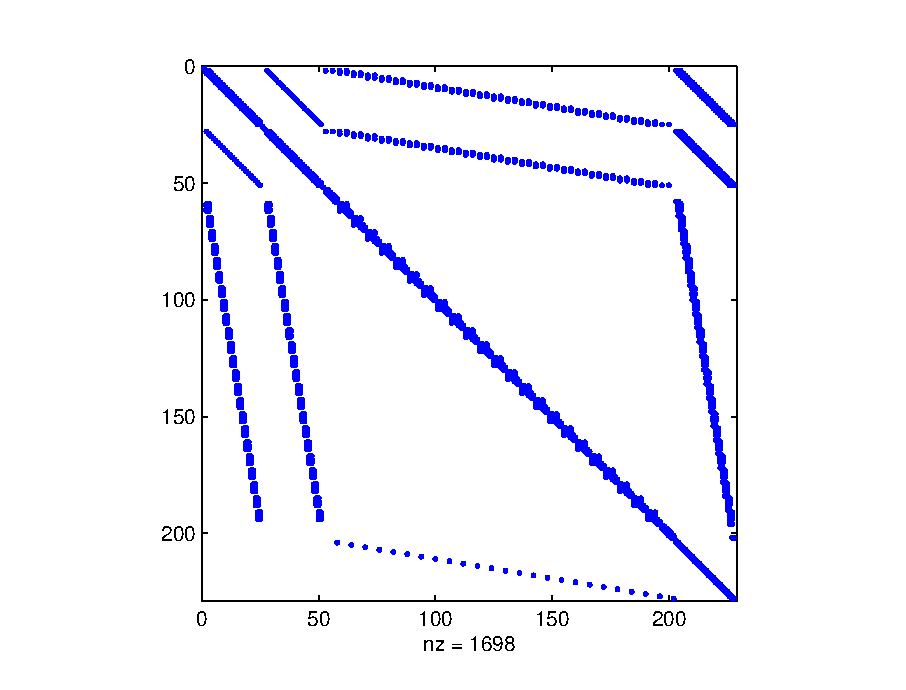
\includegraphics[scale=1.0]{J.eps}
\caption{num jac}
\end{center}
\end{figure} 

%%%%%%%%%%%%%%%%%%%%%%%%%%%%%%%%%%%%%%%%%%%%%%%%%%%%%%%%%%%%%%%%%%%%%%%%%%%%%%%%%%%%%%%%
%%%%%%%%%%%%%%%%%%%%%%%%%%%%%%%%%%%%%%%%%%%%%%%%%%%%%%%%%%%%%%%%%%%%%%%%%%%%%%%%%%%%%%%%


%%%%%%%%%%%%%%%%%%%%%%%%%%%%%%%%%%%%%%%%%%%%%%%%%%%%%%%%%%%%%%%%%%%%%%%%%%%%%%%%%%%%%%%%
%%%%%%%%%%%%%%%%%%%%%%%%%%%%%%%%%%%%%%%%%%%%%%%%%%%%%%%%%%%%%%%%%%%%%%%%%%%%%%%%%%%%%%%%
%------------------------------------------------------
\end{document}
